%% img/NPClass/SATLIP.tex
%% Copyright 2019 Andrea Berlingieri
%
% This work may be distributed and/or modified under the
% conditions of the LaTeX Project Public License, either version 1.3
% of this license or (at your option) any later version.
% The latest version of this license is in
%   http://www.latex-project.org/lppl.txt
% and version 1.3 or later is part of all distributions of LaTeX
% version 2005/12/01 or later.
%
% This work has the LPPL maintenance status `maintained'.
%
% The Current Maintainer of this work is Andrea Berlingieri.
%
% This work consists of all files listed in manifest.txt
\documentclass{standalone}

\usepackage{../TikzStyle}
\usepackage{../mystyle}
%\usetikzlibrary{decorating}
\usetikzlibrary{positioning}

\begin{document}
    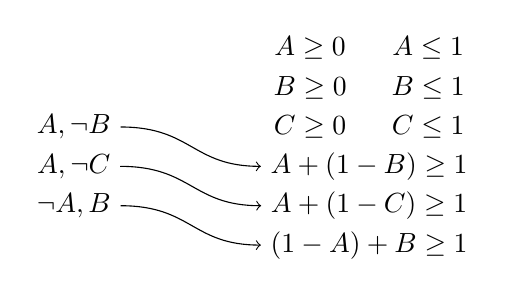
\begin{tikzpicture}[point/.style={draw,circle,inner sep=0cm,fill=black,minimum size=2pt}]
        \node (n1) at (0,0) {$\set{A,\lnot B}$};
        \node (n2) at (0,-0.5) {$\set{A,\lnot C}$};
        \node (n3) at (0,-1) {$\set{\lnot A, B}$};
        \node () at (3,1) {$A \geq 0$};
        \node () at (3,0.5) {$B \geq 0$};
        \node () at (3,0) {$C \geq 0$};
        \node () at (4.5,1) {$A \leq 1$};
        \node () at (4.5,0.5) {$B \leq 1$};
        \node () at (4.5,0) {$C \leq 1$};
        \node (n11) at (3.75,-0.5) {$A + (1-B) \geq 1$};
        \node (n22) at (3.75,-1) {$A + (1-C) \geq 1$};
        \node (n33) at (3.75,-1.5) {$(1-A)+ B \geq 1$};
        \draw[->] (n1.east) .. controls (1.5,0) and (1.5,-0.5) .. (n11.west);
        \draw[->] (n2.east) .. controls (1.5,-0.5) and (1.5,-1) .. (n22.west);
        \draw[->] (n3.east) .. controls (1.5,-1) and (1.5,-1.5) .. (n33.west);
    \end{tikzpicture}
\end{document}
